%%%%%%%%%%%%%%%%%%%%%%%%%%%%%%%%%%%%%%%%%%%%%%%%%%%
%% P3: Phenomenology of Particle Physics                         
%%
%% Author:  André Rubbia                   		 
%%
%% Figure 28.8 (left) Neutrino momentum sphere in the case of pions. (right) The correlation between
%% the neutrino energy $E_\nu$ and the parent pion energy $E_\pi$
%%
%% This work is licensed under the Creative Commons Attribution 4.0 International License. 
%% To view a copy of this license, visit http://creativecommons.org/licenses/by/4.0/ or 
%% send a letter to Creative Commons, PO Box 1866, Mountain View, CA 94042, USA.
%%
%%%%%%%%%%%%%%%%%%%%%%%%%%%%%%%%%%%%%%%%%%%%%%%%%%%

\documentclass[a4paper,10pt]{article}

\usepackage[T1]{fontenc}
\usepackage[utf8]{inputenc}
\usepackage{lmodern}
\usepackage[labelfont=bf]{caption}
\usepackage{upgreek}

\usepackage{listings}

\usepackage{tikz}
\usepackage{pgfplots}
\pgfplotsset{compat=1.17}
\usepgfplotslibrary{ternary}
\usepgfplotslibrary{fillbetween}
\usepgfplotslibrary{external}

\def\d{\mathrm{d}}
\setlength{\oddsidemargin}{-1.0cm}
\setlength{\evensidemargin}{-1.0cm}
\setlength{\textheight}{25cm}
\setlength{\textwidth}{18cm}

\pgfkeys{/pgf/number format/.cd,1000 sep={}}

\begin{document}

%%%%%%%%%%%%%%%%   FIGURE  %%%%%%%%%%%%%%%%%%%%%%%%%%%%%%
\begin{figure}[htb]
\centering
\begin{tikzpicture}[scale=1.]
\begin{axis}[xmin=0, xmax=3,
	width=0.45\textwidth,
	ytick={-0.06,-0.03,0,0.03,0.06},
	ymin=-0.06, ymax=0.06,
	title=Pion decay,
	xlabel=$p_x^\nu$ (GeV),
	ylabel=$p_y^\nu$ (GeV),
	xmajorgrids=true,
	ymajorgrids=true]
	\draw[thick,red] (axis cs:1*0.427/2,0) ellipse (1*0.427/2 and 0.0298);
	\draw[thick,blue] (axis cs:3*0.427/2,0) ellipse (3*0.427/2 and 0.0298);
	\draw[thick,magenta] (axis cs:5*0.427/2,0) ellipse (5*0.427/2 and 0.0298);
	\draw[thick,green] (axis cs:7*0.427/2,0) ellipse (7*0.427/2 and 0.0298);
\end{axis}
\end{tikzpicture}
\begin{tikzpicture}[scale=1.]
\begin{axis}[xmin=0, xmax=40,
	width=0.45\textwidth,
	ymin=0, ymax=15,
	title=Pion decay,
	xlabel=$E_\pi$ (GeV),
	ylabel=$E_\nu$ (GeV),
	xmajorgrids=true,
	ymajorgrids=true,
	legend entries={on-axis, $0.5^\circ$ off-axis, $1^\circ$ off-axis, $2^\circ$ off-axis},
	legend pos = north west]
	\addplot[domain=0:40,blue,very thick] {0.47*x};
	\addplot[domain=0:40,red,very thick] {0.47*x/(1+(x/0.139*0.5/180*3.1415)^2)};
	\addplot[domain=0:40,magenta,very thick] {0.47*x/(1+(x/0.139*1./180*3.1415)^2)};
	\addplot[domain=0:40,cyan,very thick, samples=100] {0.47*x/(1+(x/0.139*2./180*3.1415)^2)};
\end{axis}
\end{tikzpicture}
\caption{(left) Neutrino momentum sphere in the case of pions. (right) The correlation between
the neutrino energy $E_\nu$ and the parent pion energy $E_\pi$ at different
scattering angles $\theta_\nu = 0$, $0.5^\circ$, $1^\circ$, and $2^\circ$ off-axis.}
\end{figure}
%
%%%%%%%%%%%%%%%%   END FIGURE  %%%%%%%%%%%%%%%%%%%%%%%%%%%%%%
%


\end{document}
